%%=============================================================================
%% Methodologie
%%=============================================================================

\chapter{Methodologie}
\label{ch:methodologie}

\section{De keuze van de spraakassistenten}
Er is een reden waarom Siri niet mee wordt opgenomen in dit onderzoek. Ondanks dat het Nederlands ondersteunt is het toch geen goede optie voor dit onderzoek omdat je beperkt bent in het ontwikkelen van een eigen applicatie. Apple werkt met Sirikit, een framework die je alleen kan gebruiken om Siri te verwerken in je eigen IOS-applicatie. Je kunt dus geen eigen voice-applicatie maken van scratch, maar je bent verplicht om te vertrekken vanuit een mobiele applicatie. Je kunt dus alleen een bestaande applicatie uitbreiden met een optie om aan Siri vragen te stellen die hiermee te maken hebben.

Daarnaast heb je ook nog eens de beperking dat Siri alleen kan gebruikt worden op een Apple device. Binnen het kader van dit onderzoek is het belangrijk om te testen met hetzelfde apparaat. Er moet zoveel mogelijk gewerkt worden in weinig veranderlijke omstandigheden. Om te vermijden dat de hardware een invloed heeft op de resultaten worden de assistenten gebruikt op hetzelfde toestel. Sommige resultaten kunnen namelijk afhangen van de smartphone zijn prestaties. Dezelfde beperking geldt voor Bixby, die enkel kan gebruikt worden op een smartphone van Samsung.

Er is ook gezocht naar open-source projecten. Zo bestaat er Mycroft. Het grote voordeel aan Mycroft is dat het, in tegenstelling tot Google Actions of Alexa Skills, niet gekoppeld is aan een enterprise. Het is volledig open en het kan gebruikt worden in allerlei toepassingen, van een wetenschappelijk onderzoek tot een softwareapplicatie voor een bedrijf. Je kunt de software van Mycroft zelf gaan veranderen, uitbreiden en verbeteren. Daarnaast kan je ook nog kiezen voor een apparaat waar je de Mycroft software op wilt draaien. Een gewone desktop, een auto of een Raspberry Pi zijn enkele van de mogelijkheden.
De software bestaat nog niet zo lang en helaas zijn mankementen al snel zichtbaar. Iets wat direct opvalt bij het opzetten van een Android project met Mycroft is dat de documentatie heel schaars is. Sommige stappen in de documentatie staan zelfs nog beschreven als to-do. Ze bieden wel een smart speaker aan, maar die wordt weinig verkocht.

Na eerder opgesomde redenen wordt beslist om enkel Amazon Alexa en Google Assistant verder te onderzoeken. Meer specifiek zal de Amerikaans-Engelse Alexa vergeleken worden met de Amerikaans-Engelse Google Assistant en de Nederlandstalige Google Assistant uit Nederland.

\section{Wat wordt er vergeleken}
\label{sec:vergelijking van stemgestuurde assistenten}
In het onderzoek worden de kwaliteit van spraaksynthese en de kwaliteit van spraakherkenning gemeten. Twee onmisbare functionaliteiten die de afgelopen jaren door neurale netwerken zo zijn verbeterd dat het mogelijk werd om op een aangename en natuurlijke manier met spraakassistenten te communiceren. Uitgebreide informatie over \gls{STT} en \gls{TTS} is beschreven in \ref{s:spraakgestuurde technologie}.

om de kwaliteit van de spraaksynthese te meten worden er vijf eigenschappen onderscheiden die hier aan meedragen. De gebruiker beoordeelt elke assistent na het beluisteren van drie antwoorden op deze eigenschappen. Deze zijn verstaanbaarheid, menselijkheid, levendigheid, tempo en emotionaliteit. Ze zijn gekozen met het oog op een EHBO-applicatie waar het belangrijk is dat de instructies goed worden verstaan. De gebruiker moet kunnen luisteren naar een stem die klinkt als een mens en niet als een robot. De instructies mogen niet te snel en niet te traag uitgesproken worden. De levendigheid en het gevoel die aanwezig zijn in de stem van de assistent zullen ook een positieve invloed hebben op de spraakkwaliteit. De deelnemers beoordelen deze eigenschappen met de likertschaal, waarbij een score wordt gegeven van 1 tot 5. Wie de details over deze eigenschappen en hoe ze worden beoordeeld wilt kennen, kan de vragenlijst inkijken waar naar wordt verwezen in \ref{ss:deel één: met de deelnemer}.

Om te vergelijken hoe goed de assistenten spraak kunnen omvormen naar tekst, wordt er gemeten hoe sterk een bepaalde vraag die een gebruiker heeft gesteld verschilt van de zin die de assistent er van heeft gemaakt. Die sterkte wordt uitgedrukt in aantal fouten. Een fout wordt gezien als een woord uit de originele vraag die niet is opgenomen in de gevormde zin van de assistent.

\section{Gebruikte materialen}
Voor het onderzoek zijn volgende zaken gebruikt:
\begin{itemize}
    \item Acer Aspire F 15 laptop
    \begin{itemize}
        \item Intel Core I5
        \item geïntegreerde microfoon
        \item 2,5 jaar in gebruik
    \end{itemize}
    \item Xiami Redmi note 4 smartphone
    \begin{itemize}
        \item Android 7.0
        \item Octa core processor
        \item 4 GB RAM
        \item 2 jaar in gebruik
    \end{itemize}
    \item Ultimate Ears BOOM 2 Speaker
    \begin{itemize}
        \item 12,5 watt vermogen
        \item 90dB gevoeligheid
        \item 3,5mm mini-jack (AUX) ingang
        \item 1,5 jaar in gebruik
    \end{itemize}
    \item 3.5mm Jack kabel
    \item Google Assistant app voor Android
    \item Alexa Beta app voor Android
\end{itemize}

\section{Het verloop van het onderzoek}
\subsection{Deel één: met de deelnemer}
\label{ss:deel één: met de deelnemer}
De steekproef bestaat uit 30 Vlamingen tussen 19 en 60 jaar die Nederlands spreken als moedertaal en enige kennis hebben van de Engelse taal. Het onderzoek is afgenomen in twee grote delen.

De onderzoeker volgt voor dit deel een vast stappenplan die te vinden is onder onderzoek/stappenplan in de repository beschreven in \ref{s:verwijzing naar repository}.
De vragenlijst die tijdens dit deel wordt ingevuld is te vinden onder bijlagen/formulier-spraakkwaliteit in de repository beschreven in \ref{s:verwijzing naar repository}.
Er is een kleine applicatie ontwikkeld voor elke assistent waar de gebruiker drie vaste EHBO-gerelateerde vragen kan stellen en telkens een vast antwoord terugkrijgt. De applicaties voor de Google Assistant zijn ontwikkeld met DialogFlow en de Actions-On-Google console. De applicatie voor Alexa is ontwikkeld in de Alexa Developer Console. Om de juiste antwoorden te voorzien is er ook code geschreven. Het project is te vinden onder ehbo-app/testApp-ehbo-Alexa in de repository beschreven in \ref{s:verwijzing naar repository}.

\begin{figure}[H]
    \centering
    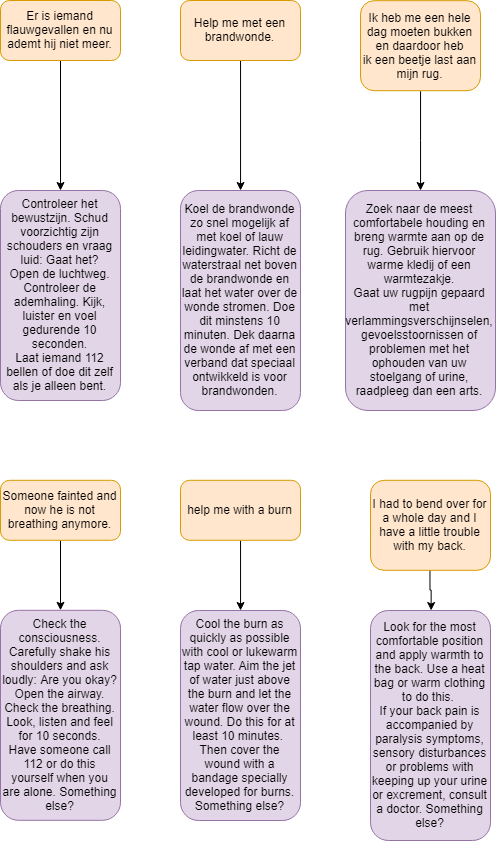
\includegraphics[width=0.7\linewidth]{img/flowdiagram_testapp}
    \caption{De flowchart waar de applicaties voor de test op zijn gebaseerd}
    \label{fig:flowdiagram}
\end{figure}

Voor het eerste deel stellen de deelnemers drie Engelse en drie Nederlandse EHBO-gerelateerde vragen aan een fictieve spraakassistent. De gestelde vragen worden opgenomen door een laptop.
Om te beginnen leest de deelnemer een korte introductietekst over spraakassistenten en vult hij enkele algemene vragen in. Daarna krijgt hij zes bladeren met op elk blad een vraag. Hij wordt aangespoord door de onderzoeker om elke vraag eerst in stilte te lezen om hem daarna te stellen aan de assistent. De aanwezigheid van een spraakassistent wordt geveinsd omdat de manier waarop de deelnemer de vragen stelt vergelijkbaar moet zijn aan de manier waarop hij ze zou stellen aan een echte assistent. De participant krijgt nooit een antwoord te horen, waardoor de mogelijkheid ontstaat dat hij steeds meer zijn best doet de volgende vraag duidelijker uit te spreken. Het verkregen resultaat zijn opgenomen audiofragmenten die later worden gebruikt in het tweede deel.

Na het stellen van alle vragen wordt de deelnemer op de hoogte gebracht van de assistent zijn afwezigheid en krijgt hij een volgende taak. Hij moet nu aan drie bestaande assistenten telkens dezelfde drie vragen stellen en te luisteren naar de drie antwoorden. Er wordt benadrukt dat het niet gaat om de inhoud van het antwoord, maar om de kwaliteit van de stem en de manier waarop het wordt gebracht. De participant krijgt de antwoorden van de assistent te horen door een speaker die met een kabel is aangesloten aan een smartphone. Hij kan de vragenlijst over de assistenten hun spraakkwaliteit al eens doornemen. De participant wordt door de onderzoeker aangespoord om goed te luisteren. Hij mag vragen opnieuw stellen tot hij antwoord krijgt van de assistent. Telkens nadat een assistent de drie vragen heeft beantwoord wordt de vragenlijst over die assistent ingevuld. De deelnemer krijgt na elke beoordeling de kans om vorige beoordelingen van assistenten aan te passen. Op het einde vult de participant nog enkele algemene vragen in.

\begin{figure}[h]
    \centering
    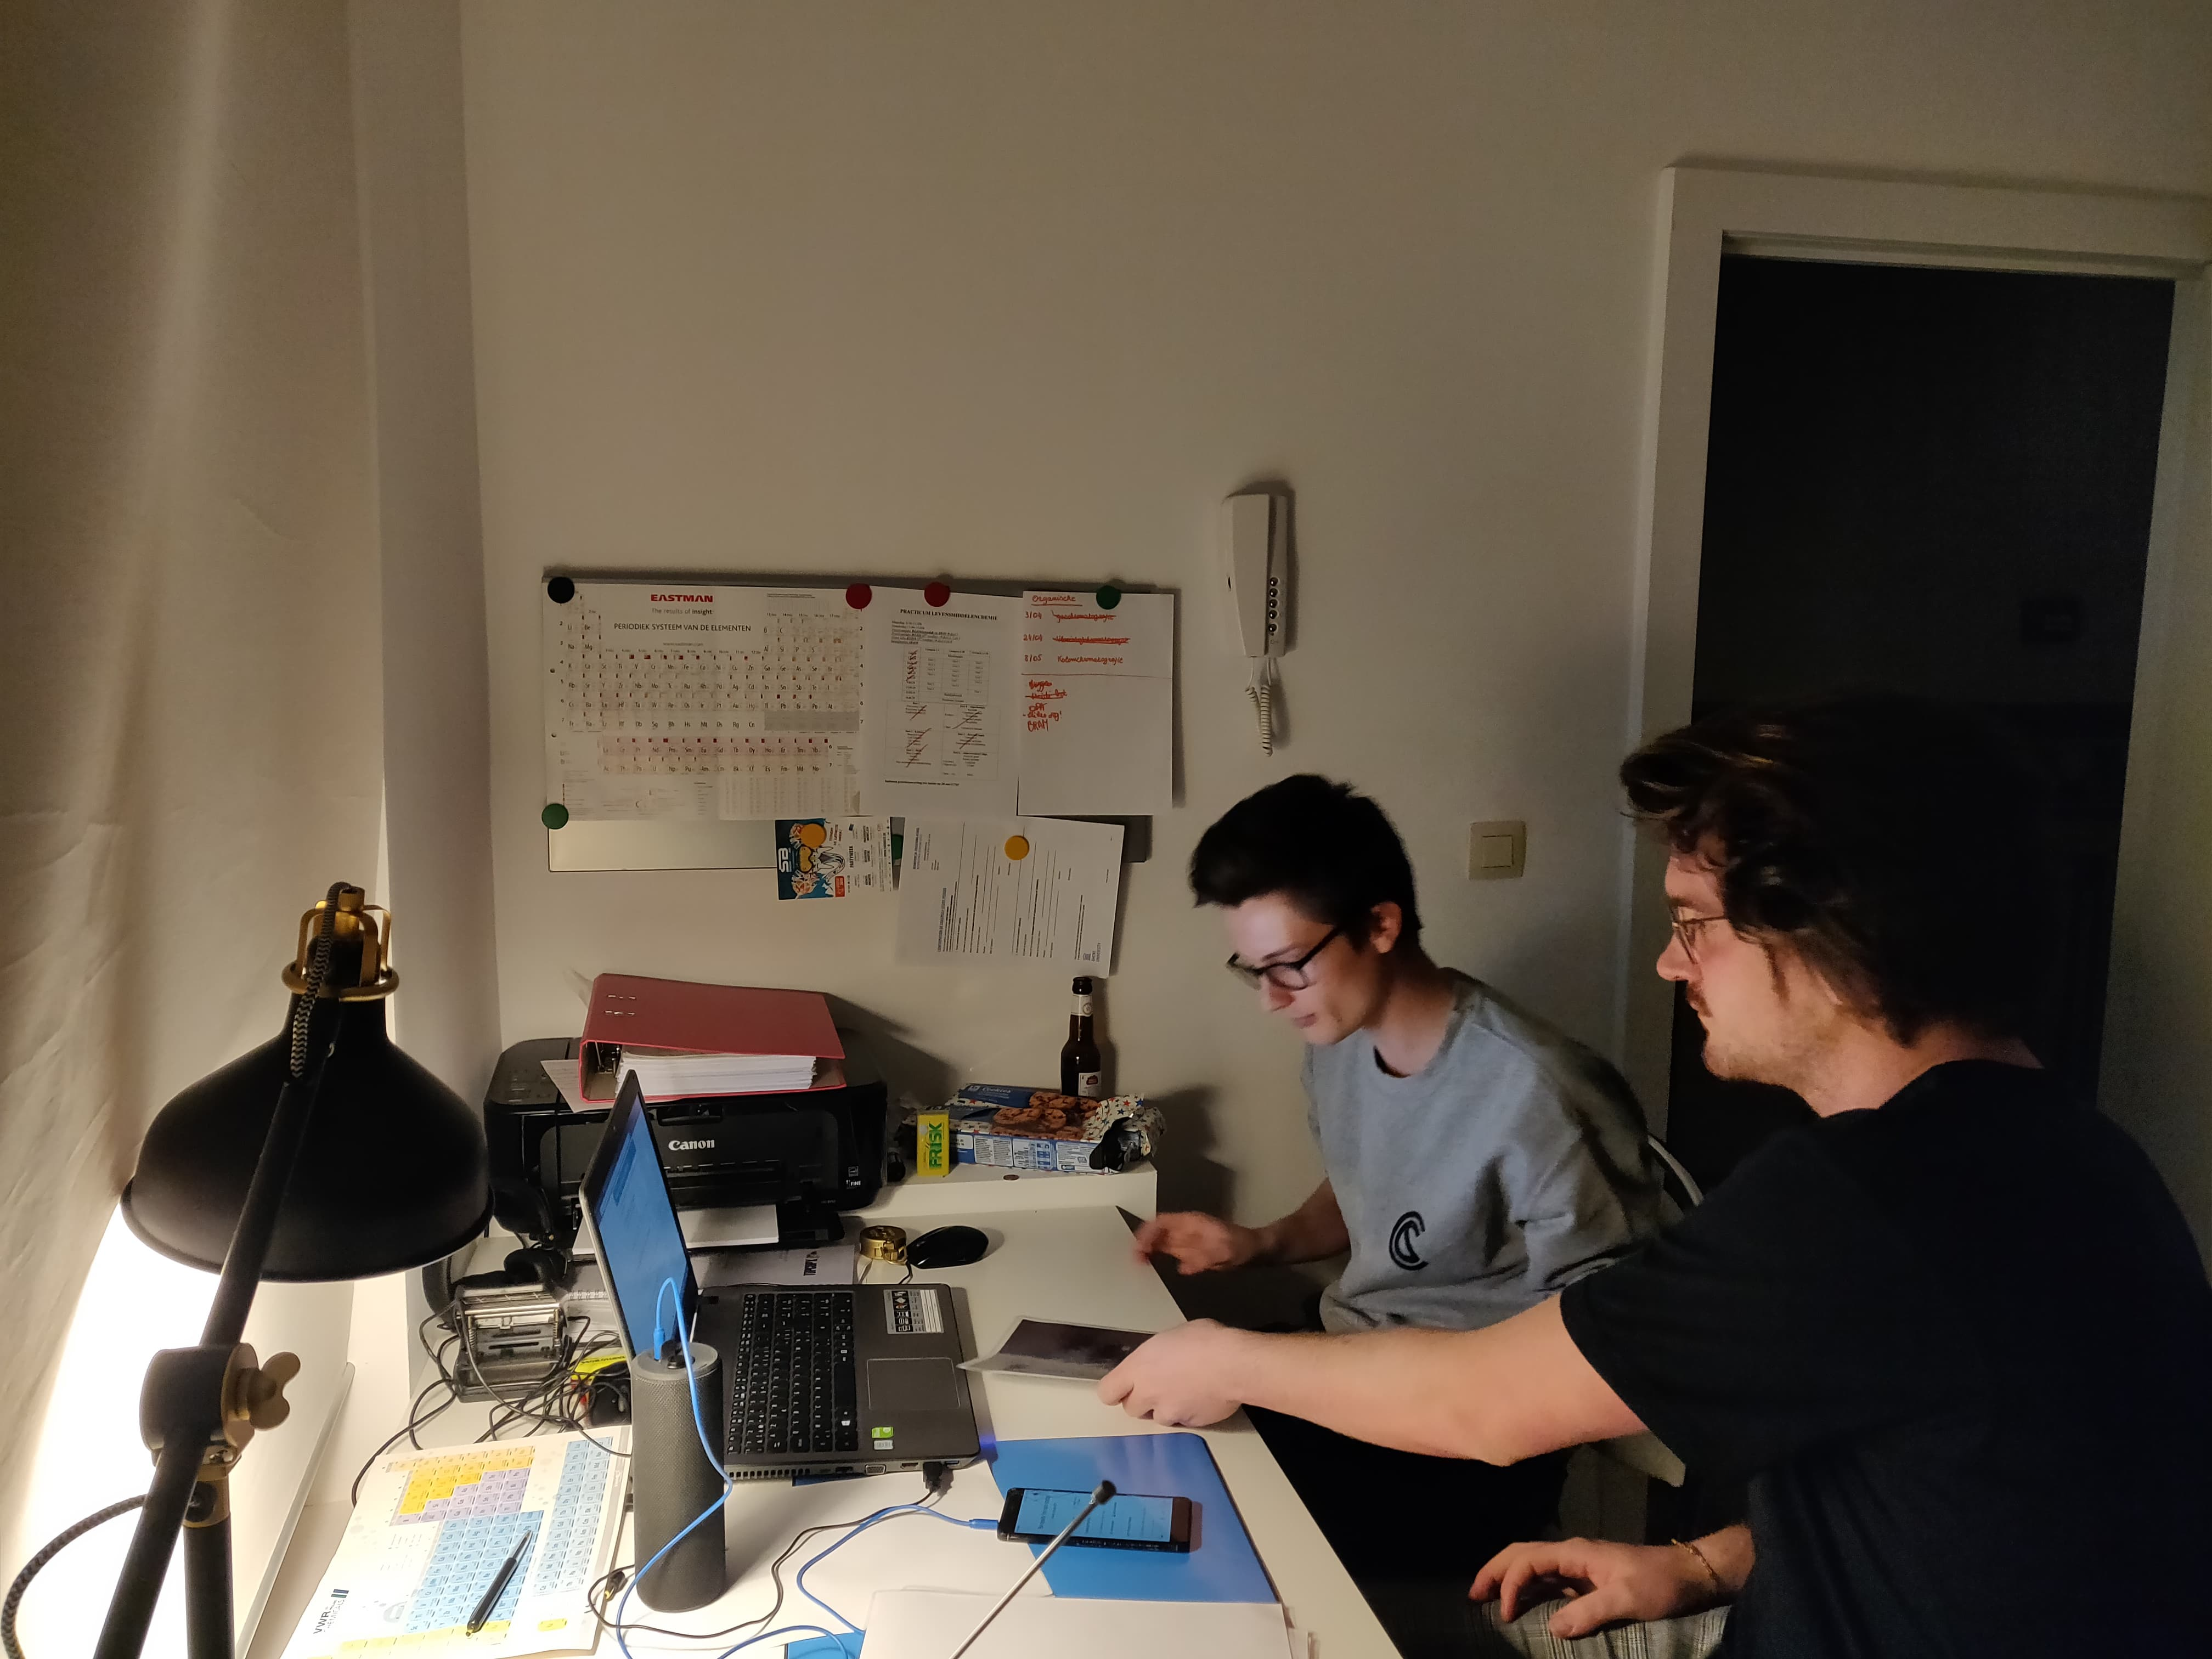
\includegraphics[width=0.7\linewidth]{img/proefafname2}
    \caption{Een deelnemer ontvangt de vragen die hij zal stellen aan de assistenten.}
    \label{fig:proefafname1}
\end{figure}

\subsection{Deel twee: zonder de deelnemer}
De vragenlijst die tijdens dit deel wordt ingevuld door de onderzoeker is te vinden onder de map bijlagen/formulier-spraakherkenning in de repository beschreven in \ref{s:verwijzing naar repository}.

Tijdens het tweede deel van het onderzoek luisteren de assistenten naar de vragen van de deelnemer. Er wordt gemeten hoe de assistenten deze vragen van spraak omzetten naar tekst. 
Er is beslist om de Nederlandse Google Assistant niet te betrekken in dit deel van het onderzoek. De reden hiervoor is dat de vragen anders zijn in het Nederlands en er figuurlijk appels zouden vergeleken worden met peren. Het aantal fouten vergelijken is niet mogelijk omdat de vertaalde vragen in het Nederlands een ander aantal woorden bevat dan de Engelse zinnen.

Er werden maatregelen genomen om de beïnvloeding van veranderlijke factoren te beperken. Zo werd tijdens het afnemen van het onderzoek beslist om de Nederlandse assistent hier niet meer bij te betrekken. De reden hiervoor was dat de Nederlandse assistent een Nederlandse vertaling van de zinnen moet herkennen, waardoor het aantal woorden in de zinnen verschillen van de Engelse zinnen. Hierdoor zou de vergelijking van het aantal fouten niet meer kloppen.

Een persoon zal ook nooit twee keer een vraag op exact dezelfde manier uitspreken. Als de deelnemer elke vraag al kan stellen zonder versprekingen dan nog zal er altijd een verschil zijn in onder meer volume, snelheid en intonatie. Daarnaast is er ook nog de extra beïnvloeding van externe ruis.
Een oplossing kan zijn om drie toestellen te gebruiken die elk voorzien zijn van een andere assistent. De gebruiker kan dan de vraag eenmalig stellen terwijl de drie assistenten tegelijkertijd luisteren. Ondanks dat dit op het eerste zicht een goede oplossing lijkt, zijn er toch enkele bedenkingen. Wegens financiële redenen is het voor de onderzoeker niet mogelijk om drie nieuwe smartphones aan te kopen. Moest dit toch mogelijk zijn dan kan er nog steeds een verschil van kwaliteit in de microfoon aanwezig zijn. Elk apparaat is uniek. Als er met drie gebruikte smartphones wordt gewerkt zal het verschil zeker aanwezig zijn door slijtage of ongelijk model.

Dit is de reden waarom de vragen zijn opgenomen in deel één. Een geregistreerd audiofragment maakt het mogelijk om de identieke vraag drie keren af te spelen terwijl telkens één assistent meeluistert op hetzelfde apparaat. Dit gebeurt in een geluidsdichte opnamestudio om externe ruis tijdens dit proces zoveel mogelijk te beperken. Er kan wel ruis mee opgenomen zijn tijdens deel één, of een deelnemer kan zich versproken hebben, maar die elementen zijn dan aanwezig bij elke assistent die het audiofragment hoort. De fragmenten worden afgespeeld door een speaker die aangesloten is op een laptop met een kabel.

\begin{figure}[H]
    \centering
    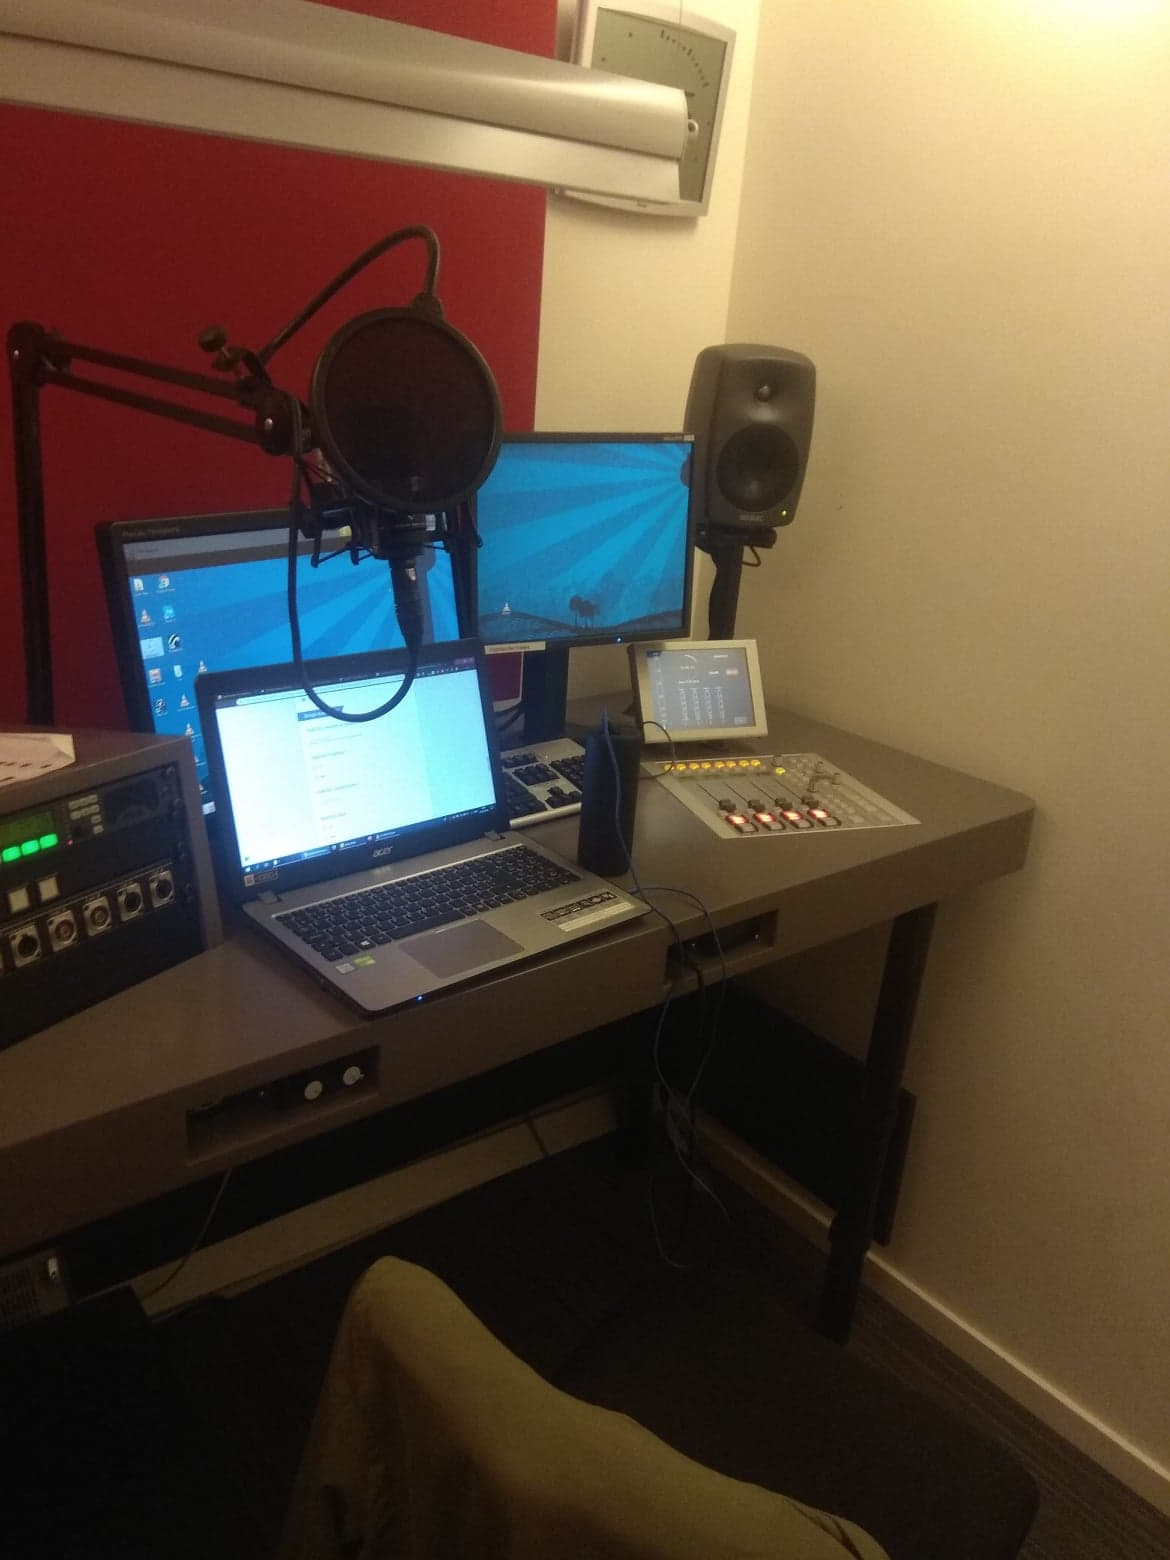
\includegraphics[width=0.7\linewidth]{img/proefafname3}
    \caption{De audiofragmenten worden beluisterd door de assistenten in een geluidsdichte studio.}
    \label{fig:proefafname2}
\end{figure}

Het is belangrijk om in achting te nemen dat de vragen niet zijn gesteld in de ontwikkelde applicaties uit deel één, maar direct aan de assistent zelf. Als je een applicatie ontwikkelt voor een spraakassistent dan verzamel je trainingszinnen zodat de applicatie weet op welke zinnen hij kan reageren. De ontwikkelaar kan uitgebreid trainingszinnen verzamelen om ervoor te zorgen dat de spraakherkenning verbeterd. Daarnaast toont Alexa in een applicatie niet altijd de rauwe tekst die hij herkent, maar soms de trainingszin die hij eraan koppelt. Het is gewoon niet duidelijk bij Alexa of hij de tekst toont die hij echt heeft begrepen of de trainingsvraag die hij er in herkent heeft. Misschien is Google wel even goed in het herkennen van een zin, maar toont Alexa direct de trainingsvraag in plaats van de tekst die hij heeft geïnterpreteerd. Om ervoor te zorgen dat de trainingszinnen geen invloed hebben op het resultaat, worden de vragen niet gesteld terwijl de applicatie is geopend. Ze worden aan de assistent zelf gesteld. Die moet het dan alleen doen met de ingebouwde speech-to-text functionaliteit en kan geen rekening houden met opgestelde trainingszinnen van de ontwikkelaar.

Zowel Alexa als Google Assistant maken het mogelijk om een overzicht van uw interacties te bekijken. Na de audiofragmenten van de 30 gebruikers af te spelen voor elke assistent werd dit overzicht gebruikt om de vragenlijst in te vullen. In de vragenlijst wordt de gevormde tekst van de assistent genoteerd samen met het aantal fouten die het bevat.